\documentclass{article}
\usepackage{graphicx}

\begin{document}
	
This is a rough working plan for RHCA tissue sampling at the HJA
\begin{center}
	\textbf{Sampling location}
\end{center}

\begin{flushleft}
	Hunter conducted surveys for RHCA in the HJA and surrounding areas in the summers of 1995 and 1996, identifying these locations.
\end{flushleft}

\begin{figure}[h]
	\centering
	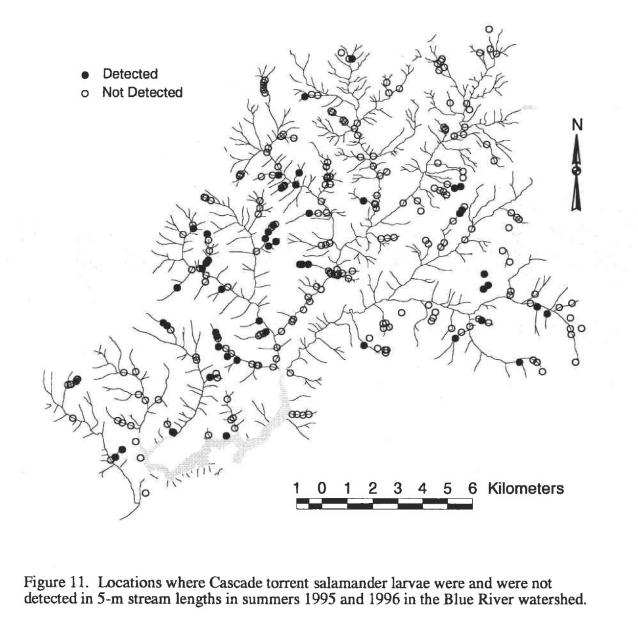
\includegraphics[scale=0.4]{Hunter.hj.results.png}
\end{figure}

\begin{flushleft}
	Hunter also used this data to model probability of occurrence.
\end{flushleft}

\begin{figure}[h]
	\centering
	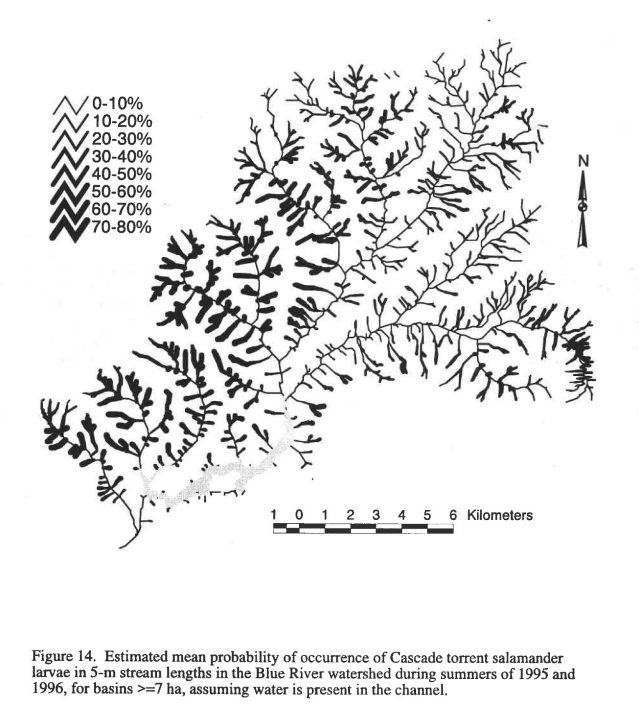
\includegraphics[scale=0.4]{Hunter.hj.probofoccurence.png}
\end{figure}

\newpage

\begin{flushleft}
	Using Hunter's thesis results and 1 vertnet observation, I've identified \textbf{8 sites} at the HJA that contain RHCA. 
\end{flushleft}

\begin{figure}[h]
	\centering
	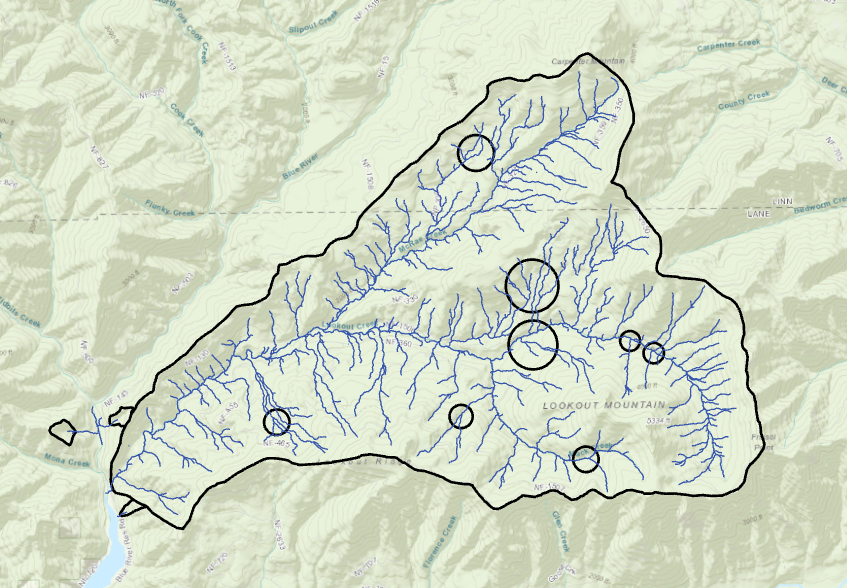
\includegraphics[scale=0.50]{HJA.sampling.map12142022.png}
\end{figure}

\end{document}
